% Make a sample document
\documentclass{article}
\usepackage{tikz}
\usetikzlibrary{calc}
\begin{document}
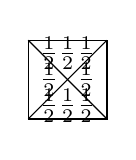
\begin{tikzpicture}
\draw (0,0) -- (1,0) -- (1,1) -- (0,1) -- cycle;
\draw (0,0) -- (1,1);
\draw (0,1) -- (1,0);
\draw (0.5,0.5) node[below] {$\frac{1}{2}$};
\draw (0.5,0.5) node[above] {$\frac{1}{2}$};
\draw (0.5,0.5) node[left] {$\frac{1}{2}$};
\draw (0.5,0.5) node[right] {$\frac{1}{2}$};
\draw (0.5,0.5) node[below left] {$\frac{1}{2}$};
\draw (0.5,0.5) node[below right] {$\frac{1}{2}$};
\draw (0.5,0.5) node[above left] {$\frac{1}{2}$};
\draw (0.5,0.5) node[above right] {$\frac{1}{2}$};
\end{tikzpicture}
\end{document}